% -*- root: ../main.tex -*-
\chapter{Design di Dettaglio}

\section{Design Gestione Cibo e Acqua}
    Per l'automatizzazione e la gestione di cibo e acqua si è partiti dalle user-stories e dal modello costruito per sviluppare l'applicativo desiderato. Osservando i requisiti è stato modellato il modello fisico e l'interazione dell'animale con esso. 
    Si riporta di seguito il design fisico, con i sensori e attuatori in giallo e la spiegazione del suo funzionamento [Fig. \ref{fig:ciboacqua}].
    Il design permette la modularità tra cibo e acqua, scegliendo all'occorrenza solo uno dei due o entrambi.
    \begin{figure}[H]
        \caption{Design Prototipo Cibo e Acqua}
        \label{fig:ciboacqua}
        \centering
        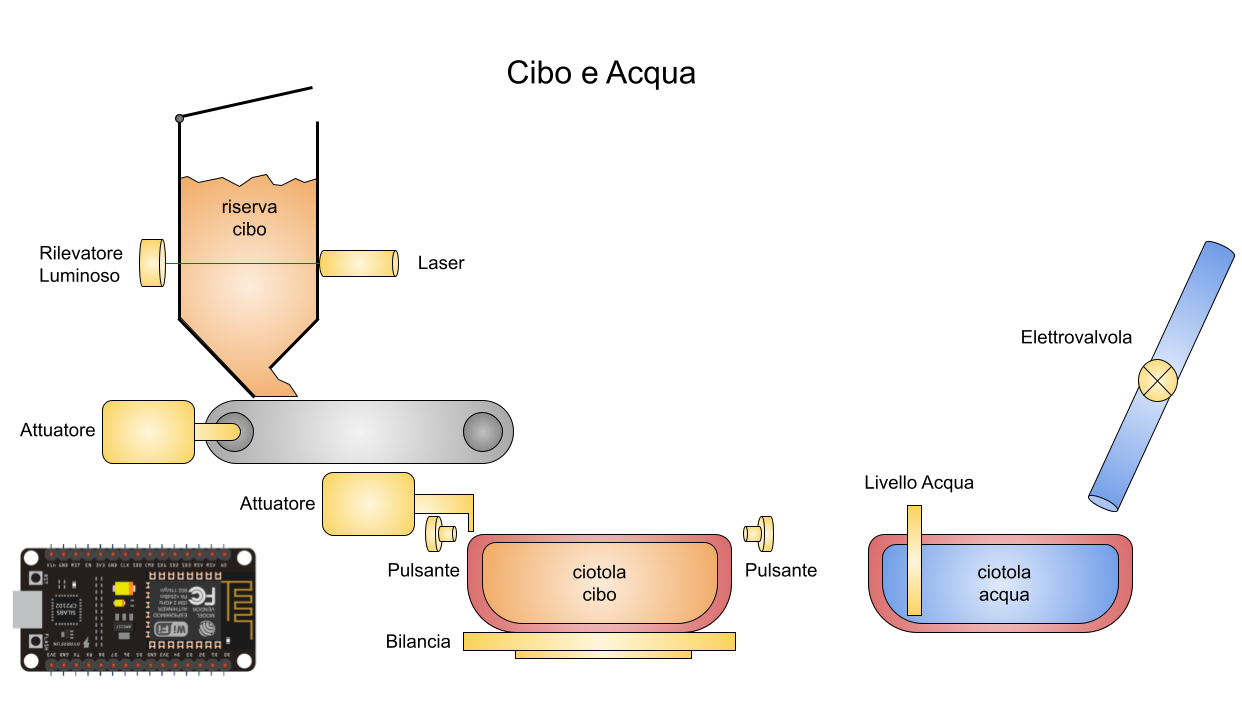
\includegraphics[width=1\textwidth]{Images/CiboAcqua.png}
    \end{figure}
    
    \subsection{Acqua}
    Per far fronte alla misurazione dei consumi, è stato innanzitutto necessario scegliere un sensore per ricavarne il livello del liquido [Fig. \ref{fig:ciboacqua}]. Il sensore deve ritornare un valore proporzionale alla percentuale di liquido rimanente. I consumi dell'animale a questo punto verranno inviati in cloud.
    
    Per quanto riguarda l'esigenza di riempimento dell'acqua, inizialmente la scelta era ricaduta su due sensori che rivelassero quando il liquido è al minimo o al massimo. In seguito questo design è stato semplificato usando direttamente il sensore introdotto per l'invio dei dati relativi al livello del liquido. 
    Successivamente è necessario che il sensore si interfacci con un'elettrovalvola [Fig. \ref{fig:ciboacqua}] per poter riempire la ciotola aprendo o chiudendo il flusso d'acqua all'occorrenza. 
    
    Il sistema deve essere modulare per design: qualora non si disponga del sistema idrico per poter rifornire la ciotola, devono comunque essere mandati i consumi con l'aggiunta di una notifica se se l'acqua sta per terminare.
    
    \subsubsection{Macchina a stati} Il comportamento è stato modellato come una macchina a stati [Fig. \ref{fig:statediagramWater}]. Ciò ha permesso di chiarire meglio le azioni del sistema a fronte di un avvenimento, il suo stato corrente e il suo comportamento generale.
    Inizialmente il comportamento prevede il controllo del consumo di acqua, ciclicamente e a intervalli regolari viene fatta una misurazione [Fig. \ref{fig:statediagramWater} "check water consumption"]. 
    E' stata stabilita una soglia minima di diminuzione del liquido per non incorrere in falsi positivi, dove le naturali oscillazioni del sensore potrebbero inviare consumi inesistenti. 
    Talora questa soglia venisse superata, la percentuale di liquido consumata viene inviata in cloud, memorizzando l'ultima percentuale inviata [Fig. \ref{fig:statediagramWater} "send water consumption"]. Il sistema continua quindi a monitorare di nuovo il livello per ulteriori consumi. 
    Inevitabilmente il liquido nella ciotola andrà a finire, questo evento innescherà una transizione, dipendente dalla presenza o meno dell'elettrovalvola. 
    Se il sistema non prevede un rifornimento idrico il sistema passerà allo stato di notifica di acqua esaurita [Fig. \ref{fig:statediagramWater} "finished water notify"]. In questo stato una notifica verrà mandata all'addetto ai rifornimenti. Quando la ciotola verrà ricaricata il sistema passerà in automatico nuovamente allo stato per il controllo dei consumi.
    Qualora il sistema fosse dotato di elettrovalvola, la transizione innescata la aprirebbe, passando allo stato di riempimento [Fig. \ref{fig:statediagramWater} "fill water bowl"]. In questo stato il livello viene controllato continuamente, per non incorrere in allagamenti indesiderati. 
    Un meccanismo di sicurezza temporizzato infatti controlla se un determinato periodo di tempo è passato senza che il sistema sia riuscito a riempire la ciotola con la valvola aperta. In caso affermativo il sistema va in blocco, chiudendo la valvola e passando allo stato di notifica di errore [Fig. \ref{fig:statediagramWater} "water system error notify"]. 
    Se il livello dell'acqua raggiunge il parametro desiderato invece lo stato torna a essere quello iniziale di osservazione.
    
    \begin{figure}[H]
        \caption{Macchina a Stati Acqua}
        \label{fig:statediagramWater}
        \centering
        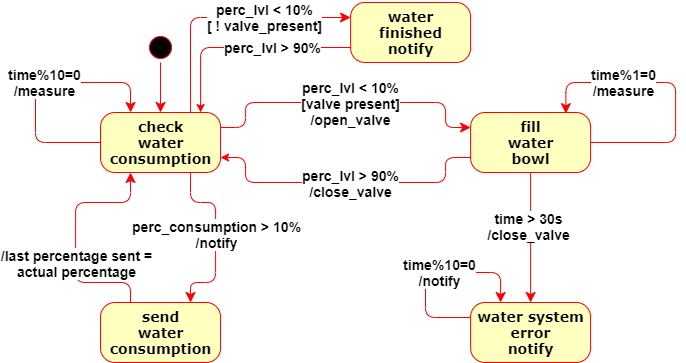
\includegraphics[width=1\textwidth]{DrawIo/stateDiagramWater.png}
    \end{figure}
    
    \subsection{Cibo}
    Per far fronte all'esigenza di monitorare i consumi di cibo dell'animale è stata introdotto un sensore di peso. Il sensore deve ritornare un valore proporzionale alla quantità di cibo presente nella ciotola. I consumi dell'animale verranno inviati in cloud. 
    
    
\section{Design Monitoraggio Parametri Vitali}

\section{Design Videosorveglianza}

\section{Design del Database}
Per immagazzinare i dati necessari all'applicazione si è deciso di utilizzare \textbf{Dynamo DB}.
Il database principale doveva immagazzinare:
\begin{itemize}
    \item I \textbf{profili} dei \textbf{cani} presenti all'interno del canile;
    \item Gli \textbf{orari} e le \textbf{quantità} di cibo da somministrare a seconda del cane;
    \item I \textbf{valori} rilevati dai dispositivi di \textbf{sensing}, che comprendono:
    \begin{itemize}
        \item Temperatura corporea;
        \item Frequenza cardiaca;
        \item Consumo di acqua; 
        \item Consumo di cibo;
        \item Temperatura ambientale del canile;
        \item Umidità rilevata all'interno del canile;
    \end{itemize}
    \item I profili degli \textbf{utenti}.
\end{itemize}

La progettazione del database è stata portata a termine seguendo diversi passaggi:
    \begin{enumerate}
        \item Definizione di uno schema \textbf{ER} da utilizzare come base di partenza;
        \item Individuazione degli \textbf{accessi} mediante la definizione delle \textbf{query} principali;
        \item Definizione dei \textbf{pattern} di Primary Key e Sort Key;
        \item Aggiunta di un \textbf{ global index};
    \end{enumerate}
    
    \subsection{Definizione di un ER}
    Nonostante non si tratti di un database relazionale, abbozzare uno schema Entity Relationship può essere utile per avere una buona visione di partenza di come devono essere gestiti i dati.
    L'elaborazione dello schema ER ha portato ai seguenti risultati:
 
     \begin{figure}[H]
        \caption{ER dati del cane}
        \label{fig:dogER}
        \centering
        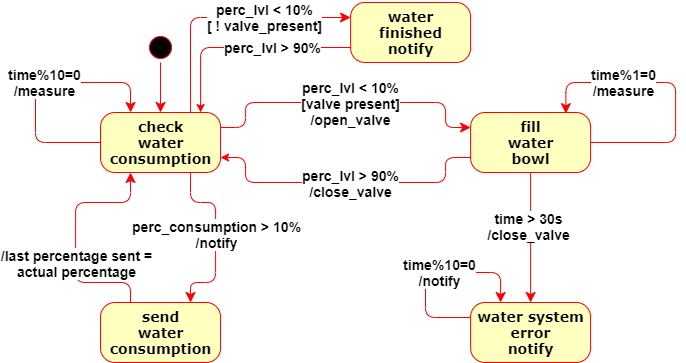
\includegraphics[width=1\textwidth]{DrawIo/stateDiagramWater.png}
    \end{figure}